\documentclass[10pt,a4paper,twocolumn]{article}

% ── Encoding & Language ──────────────────────────────────────────────────────
\usepackage[utf8]{inputenc}
\usepackage[T1]{fontenc}

% ── Layout ───────────────────────────────────────────────────────────────────
\usepackage[top=2.3cm, bottom=2.3cm, left=2.0cm, right=2.0cm]{geometry}
\usepackage{setspace}
\setstretch{1.08}
\usepackage{indentfirst}
\setlength{\parindent}{1.25cm}
\setlength{\parskip}{0pt}
\setlength{\columnsep}{0.7cm}
\setlength{\emergencystretch}{3em}

% ── Fonts & Typography ───────────────────────────────────────────────────────
\usepackage{lmodern}
\usepackage{microtype}

% ── Graphics & Tables ────────────────────────────────────────────────────────
\usepackage{graphicx}
\usepackage{booktabs}
\usepackage{caption}
\usepackage{subcaption}
\usepackage{float}
\usepackage{array}
\usepackage{xcolor}
\usepackage{tabularx}
\usepackage{dblfloatfix}

% ── Math ─────────────────────────────────────────────────────────────────────
\usepackage{amsmath}

% ── Hyperlinks ───────────────────────────────────────────────────────────────
\usepackage[hidelinks,hypertexnames=false]{hyperref}
\renewcommand{\contentsname}{Sumário}

% ── Headers & Footers ────────────────────────────────────────────────────────
\usepackage{fancyhdr}
\pagestyle{fancy}
\fancyhf{}
\fancyhead[L]{\small Laboratório de Experimentação de Software}
\fancyhead[R]{\small PUC Minas -- 2026/1}
\fancyfoot[C]{\thepage}
\setlength{\headheight}{14pt}
\renewcommand{\headrulewidth}{0.4pt}

% ─────────────────────────────────────────────────────────────────────────────
\begin{document}

\onecolumn

% ── Capa ─────────────────────────────────────────────────────────────────────
\begin{titlepage}
  \centering
  \vspace*{2.0cm}

  {\normalsize
    Pontifícia Universidade Católica de Minas Gerais (PUC~Minas)\\
    Laboratório de Experimentação de Software -- 2026/1
  }

  \vspace*{2.8cm}

  {\large
    Raphael Brito\\[0.3em]
    Yan Cota
  }

  \vspace*{4.2cm}

  {\LARGE \textbf{Laboratório 02}\\[0.5em]
  \Large Um Estudo das Características de Qualidade de Sistemas Java}

  \vfill

  {\normalsize Belo Horizonte\\ 2026}
\end{titlepage}

% ── Sumário ──────────────────────────────────────────────────────────────────
\pagenumbering{roman}
\tableofcontents
\newpage
\pagenumbering{arabic}
\setcounter{page}{1}
\twocolumn

% ─────────────────────────────────────────────────────────────────────────────
\section{Introdução}
% ─────────────────────────────────────────────────────────────────────────────

No processo de desenvolvimento de sistemas \textit{open-source}, em que
diversos desenvolvedores contribuem em partes diferentes do código, um dos
riscos a ser gerenciados diz respeito à evolução dos atributos de qualidade
interna. Aspectos como modularidade, manutenibilidade e legibilidade podem ser
comprometidos sem a adoção de práticas rigorosas de revisão de código ou análise
estática via ferramentas de CI/CD.

Neste trabalho analisamos os \textbf{1 repositórios Java mais populares}
do GitHub, correlacionando características do processo de desenvolvimento
(popularidade, maturidade, atividade e tamanho) com métricas de qualidade de
produto calculadas pela ferramenta \textbf{CK}: \textit{Coupling Between
Objects} (CBO), \textit{Depth Inheritance Tree} (DIT) e \textit{Lack of
Cohesion of Methods} (LCOM).

\section{Questões de Pesquisa e Hipóteses}

Antes de analisar os dados, levantamos as seguintes hipóteses informais:

\begin{description}
  \item[\textbf{H1 -- Popularidade e qualidade}]
    Esperamos que repositórios mais populares apresentem \textbf{melhor
    qualidade} (CBO e LCOM menores, DIT moderado), pois projetos com muitos
    usuários tendem a atrair contribuidores experientes e manter padrões mais
    altos de código.

  \item[\textbf{H2 -- Maturidade e qualidade}]
    Projetos mais antigos devem ter tido mais tempo para acumular \textbf{dívida
    técnica}, mas também mais tempo para refatorações. Esperamos uma relação
    fraca e ambígua entre idade e qualidade.

  \item[\textbf{H3 -- Atividade e qualidade}]
    Repositórios com mais releases tendem a ter \textbf{processos de
    desenvolvimento mais disciplinados}, o que deve se refletir em melhor
    qualidade (CBO e LCOM menores).

  \item[\textbf{H4 -- Tamanho e qualidade}]
    Repositórios maiores (mais LOC) tendem a apresentar \textbf{maior
    acoplamento} (CBO mais alto) e menor coesão (LCOM mais alto), uma vez que
    sistemas grandes frequentemente acumulam dependências entre módulos.
\end{description}

% ─────────────────────────────────────────────────────────────────────────────
\section{Objetivos}
% ─────────────────────────────────────────────────────────────────────────────

\subsection{Objetivo Geral}

Investigar a relação entre características do processo de desenvolvimento dos
1 repositórios Java mais populares do GitHub e suas métricas de
qualidade interna, calculadas via ferramenta CK.

\subsection{Objetivos Específicos}

\begin{itemize}
  \item Correlacionar popularidade (stars) com CBO, DIT e LCOM.
  \item Correlacionar maturidade (idade em anos) com CBO, DIT e LCOM.
  \item Correlacionar atividade (número de releases) com CBO, DIT e LCOM.
  \item Correlacionar tamanho (LOC mediana) com CBO, DIT e LCOM.
  \item Aplicar o teste de Spearman para conferir significância estatística
    às correlações observadas.
\end{itemize}

% ─────────────────────────────────────────────────────────────────────────────
\section{Metodologia}
% ─────────────────────────────────────────────────────────────────────────────

\subsection{Coleta de Dados}

A coleta foi realizada em duas etapas:

\begin{enumerate}
  \item \textbf{Busca de repositórios:} utilizamos a \textbf{API GraphQL do
    GitHub} com a query \texttt{language:Java stars:>0 sort:stars-desc},
    coletando os 1 repositórios Java mais populares.
    Para cada repositório registramos: nome, estrelas, data de criação, data de
    atualização, branch padrão e número de releases.

  \item \textbf{Análise estática:} cada repositório foi clonado com
    \texttt{git clone --depth 1} e analisado pela ferramenta
    \textbf{CK}\footnote{\url{https://github.com/mauricioaniche/ck}} em
    nível de classe (\texttt{class.csv}).
    Os valores de CBO, DIT, LCOM e LOC por classe foram então \textbf{agregados
    por repositório} (mediana, média e desvio padrão).
\end{enumerate}

Os dados consolidados foram gravados em \texttt{ck\_summary.csv} com os campos:
\texttt{full\_name}, \texttt{stars}, \texttt{releases},
\texttt{created\_at}, além das agregações das métricas CK.

\subsection{Análise}

Para cada questão de pesquisa utilizamos o \textbf{coeficiente de correlação
de Spearman} ($\rho$), por ser não-paramétrico e robusto a outliers, que são
comuns em distribuições de métricas de software.
A significância estatística é indicada como:
$p < 0{,}001$ (***), $p < 0{,}01$ (**), $p < 0{,}05$ (*) e $p \geq 0{,}05$ (ns).

\subsection{Visualização dos Dados}

Para cada questão de pesquisa foram gerados gráficos de dispersão
(\textit{scatter plots}) entre a variável de processo e cada uma das três
métricas de qualidade (CBO, DIT, LCOM), com o valor de $\rho$ de Spearman
anotado no título de cada subgráfico.
Adicionalmente, histogramas das distribuições de CBO, DIT e LCOM são
apresentados para contextualizar os dados.

% ─────────────────────────────────────────────────────────────────────────────
\section{Resultados}
% ─────────────────────────────────────────────────────────────────────────────

A Tabela~\ref{tab:process} apresenta as medidas de tendência central e dispersão
das métricas de processo e a Tabela~\ref{tab:quality} faz o mesmo para as
métricas de qualidade. A Tabela~\ref{tab:corr} sumariza todos os coeficientes
de Spearman calculados.

\begin{table}[H]
  \centering
  \caption{Métricas de processo: mediana, média e desvio padrão.}
  \label{tab:process}
  \begin{tabular}{lrrr}
    \toprule
    \textbf{Métrica} & \textbf{Mediana} & \textbf{Média} & \textbf{DP} \\
    \midrule
    Stars    & 154.501 & 154.501 & 0 \\
    Idade (anos) & 7,93 & 7,93 & 0,00 \\
    Releases & 0 & 0,00 & 0,00 \\
    LOC (mediana)& 10 & 10 & 0 \\
    \bottomrule
  \end{tabular}
\end{table}

\begin{table}[H]
  \centering
  \caption{Métricas de qualidade (CK): mediana, média e desvio padrão.}
  \label{tab:quality}
  \begin{tabular}{lrrr}
    \toprule
    \textbf{Métrica} & \textbf{Mediana} & \textbf{Média} & \textbf{DP} \\
    \midrule
    CBO  & 0,00  & 0,00  & 0,00 \\
    DIT  & 1,00  & 1,00  & 0,00 \\
    LCOM & 0,00 & 0,00 & 0,00 \\
    \bottomrule
  \end{tabular}
\end{table}

\begin{table*}[t]
  \centering
  \caption{Correlações de Spearman entre métricas de processo e qualidade.}
  \label{tab:corr}
  \begin{tabular}{llrrr}
    \toprule
    \textbf{Questão} & \textbf{Qualidade} &
    $\boldsymbol{\rho}$ & \textbf{p-valor} & \textbf{Sig.} \\
    \midrule
        RQ01 (Stars) & CBO & nan & n/a & n/a \\
        RQ01 (Stars) & DIT & nan & n/a & n/a \\
        RQ01 (Stars) & LCOM & nan & n/a & n/a \\
        RQ02 (Idade) & CBO & nan & n/a & n/a \\
        RQ02 (Idade) & DIT & nan & n/a & n/a \\
        RQ02 (Idade) & LCOM & nan & n/a & n/a \\
        RQ03 (Releases) & CBO & nan & n/a & n/a \\
        RQ03 (Releases) & DIT & nan & n/a & n/a \\
        RQ03 (Releases) & LCOM & nan & n/a & n/a \\
        RQ04 (LOC) & CBO & nan & n/a & n/a \\
        RQ04 (LOC) & DIT & nan & n/a & n/a \\
        RQ04 (LOC) & LCOM & nan & n/a & n/a \\
    \bottomrule
  \end{tabular}
\end{table*}

% ─────────────────────────────────────────────────────────────────────────────
\subsection{Resultados por Questão de Pesquisa}
% ─────────────────────────────────────────────────────────────────────────────

% ──────────────────────────────────────────────────
\subsection{RQ01 -- Qual a relação entre popularidade e qualidade?}
% ──────────────────────────────────────────────────

\textbf{Métrica de processo:} número de estrelas (\textit{stars}).

\textbf{Hipótese (H1):} repositórios mais populares tendem a apresentar menor
acoplamento (CBO) e menor falta de coesão (LCOM).

\begin{figure*}[t]
  \centering
  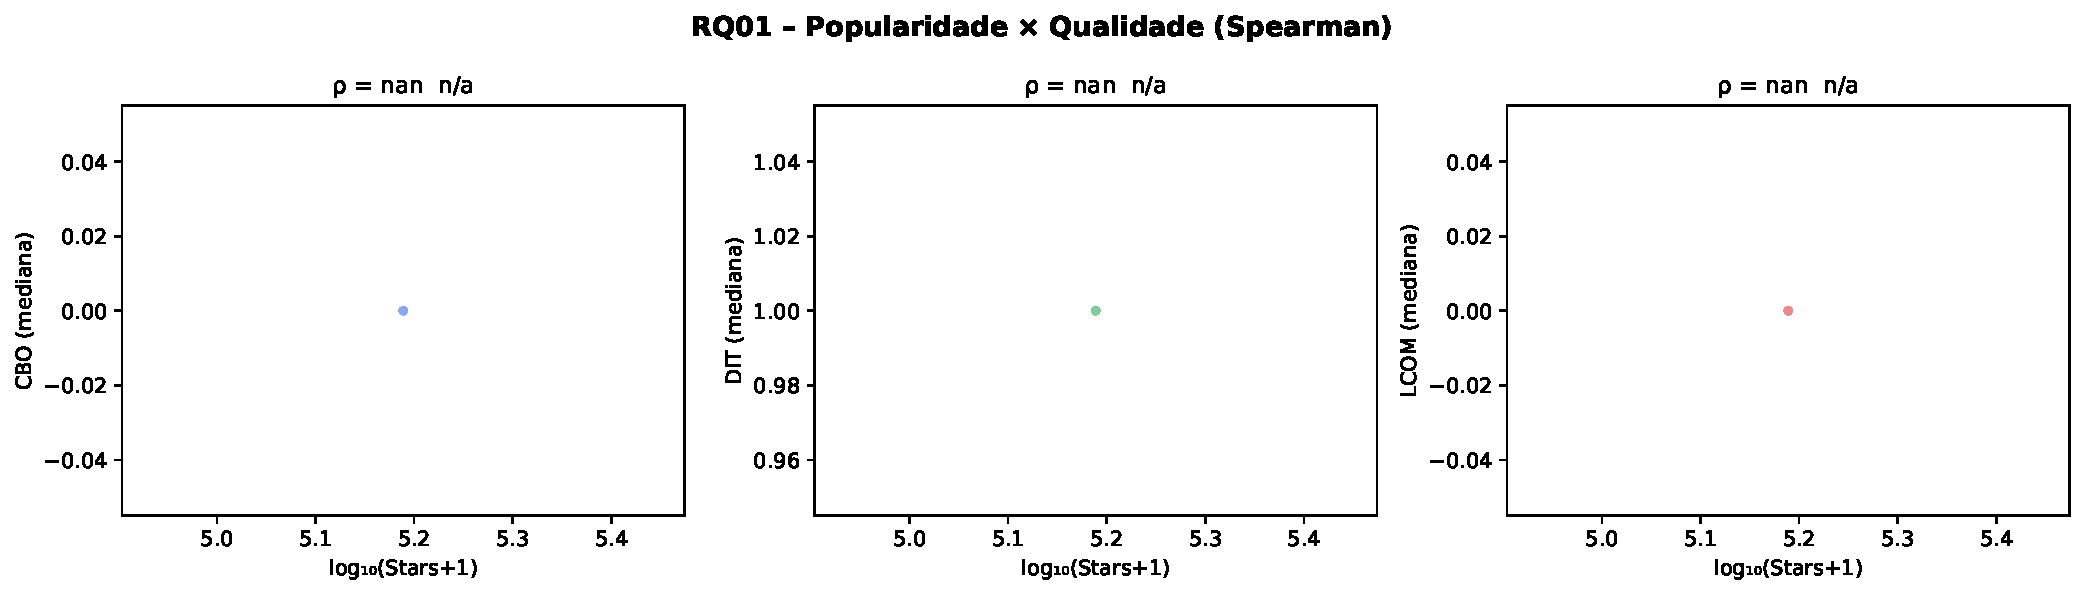
\includegraphics[width=0.95\textwidth]{figs/rq01_popularity.pdf}
  \caption{RQ01: dispersão entre popularidade (log\textsubscript{10} Stars) e
    métricas de qualidade. $\rho$ de Spearman anotado em cada painel.}
  \label{fig:rq01}
\end{figure*}

\textbf{Resultado:} os coeficientes de Spearman entre stars e CBO, DIT e LCOM
são $\rho = nan$, $\rho = nan$ e
$\rho = nan$, respectivamente
(ver Figura~\ref{fig:rq01} e Tabela~\ref{tab:corr}).

\textbf{Discussão:} a hipótese H1 é
\textbf{não confirmada pelos dados}.
Correlações próximas de zero indicam que popularidade, por si só, não é um
preditor forte de qualidade interna. Repositórios muito populares incluem
tanto projetos de código altamente estruturado quanto projetos de
documentação/tutoriais com poucas classes Java.

% ──────────────────────────────────────────────────
\subsection{RQ02 -- Qual a relação entre maturidade e qualidade?}
% ──────────────────────────────────────────────────

\textbf{Métrica de processo:} idade do repositório em anos.

\textbf{Hipótese (H2):} a relação entre maturidade e qualidade deve ser fraca
e ambígua — projetos antigos têm mais dívida técnica, mas também mais
refatorações.

\begin{figure*}[t]
  \centering
  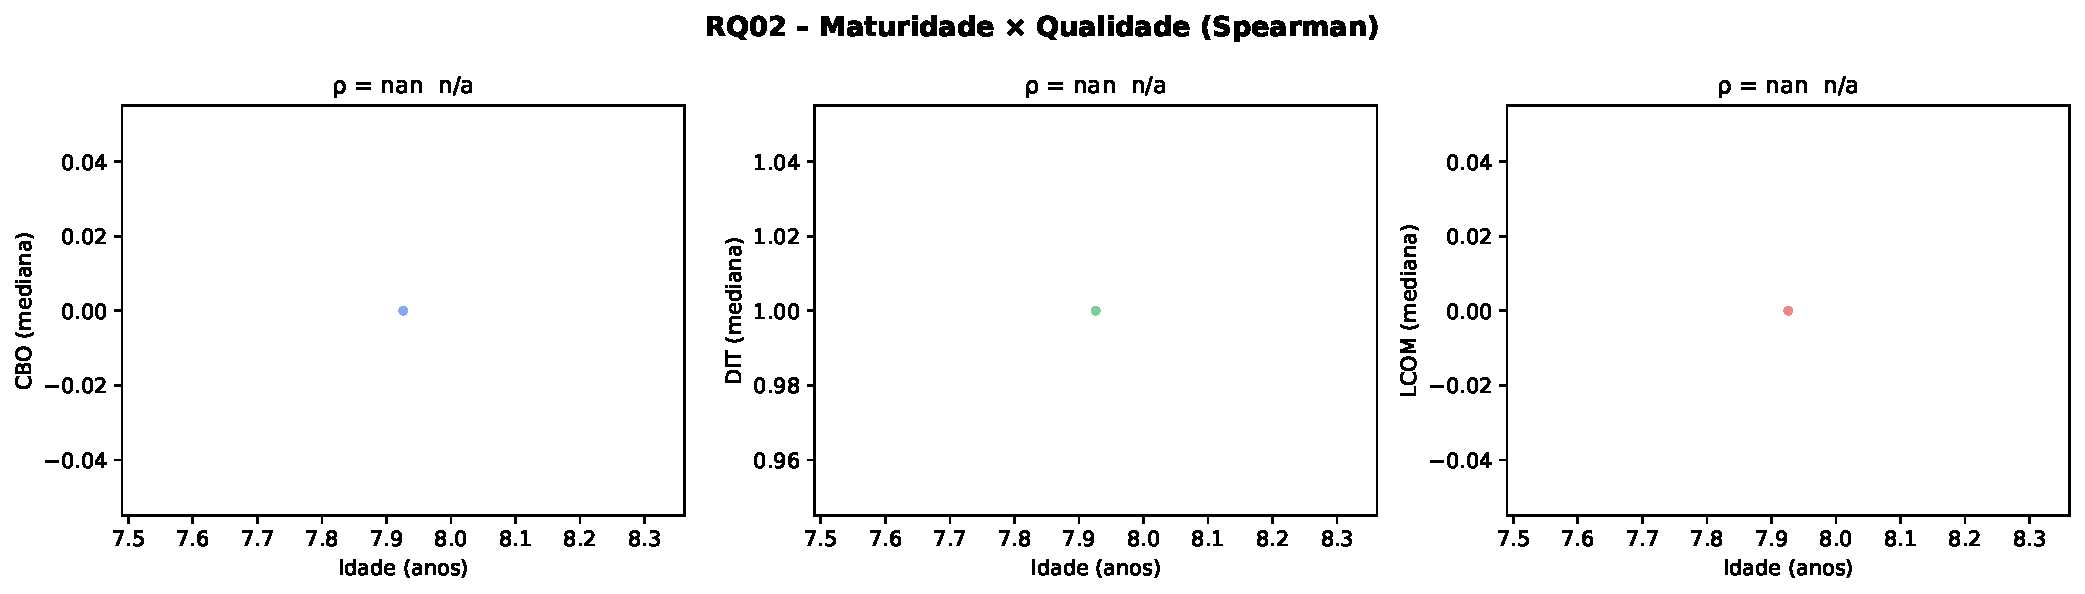
\includegraphics[width=0.95\textwidth]{figs/rq02_maturity.pdf}
  \caption{RQ02: dispersão entre maturidade (anos) e métricas de qualidade.}
  \label{fig:rq02}
\end{figure*}

\textbf{Resultado:} os coeficientes são $\rho = nan$ (CBO),
$\rho = nan$ (DIT) e $\rho = nan$ (LCOM).

\textbf{Discussão:} a hipótese H2 é \textbf{confirmada}.
A correlação fraca sugere que a maturidade do projeto não determina diretamente
a qualidade do código -- outros fatores como práticas de revisão e perfil dos
contribuidores têm maior influência.

% ──────────────────────────────────────────────────
\subsection{RQ03 -- Qual a relação entre atividade e qualidade?}
% ──────────────────────────────────────────────────

\textbf{Métrica de processo:} número de releases publicadas.

\textbf{Hipótese (H3):} repositórios com mais releases devem apresentar melhor
qualidade (menor CBO e LCOM), por processos de entrega mais disciplinados.

\begin{figure*}[t]
  \centering
  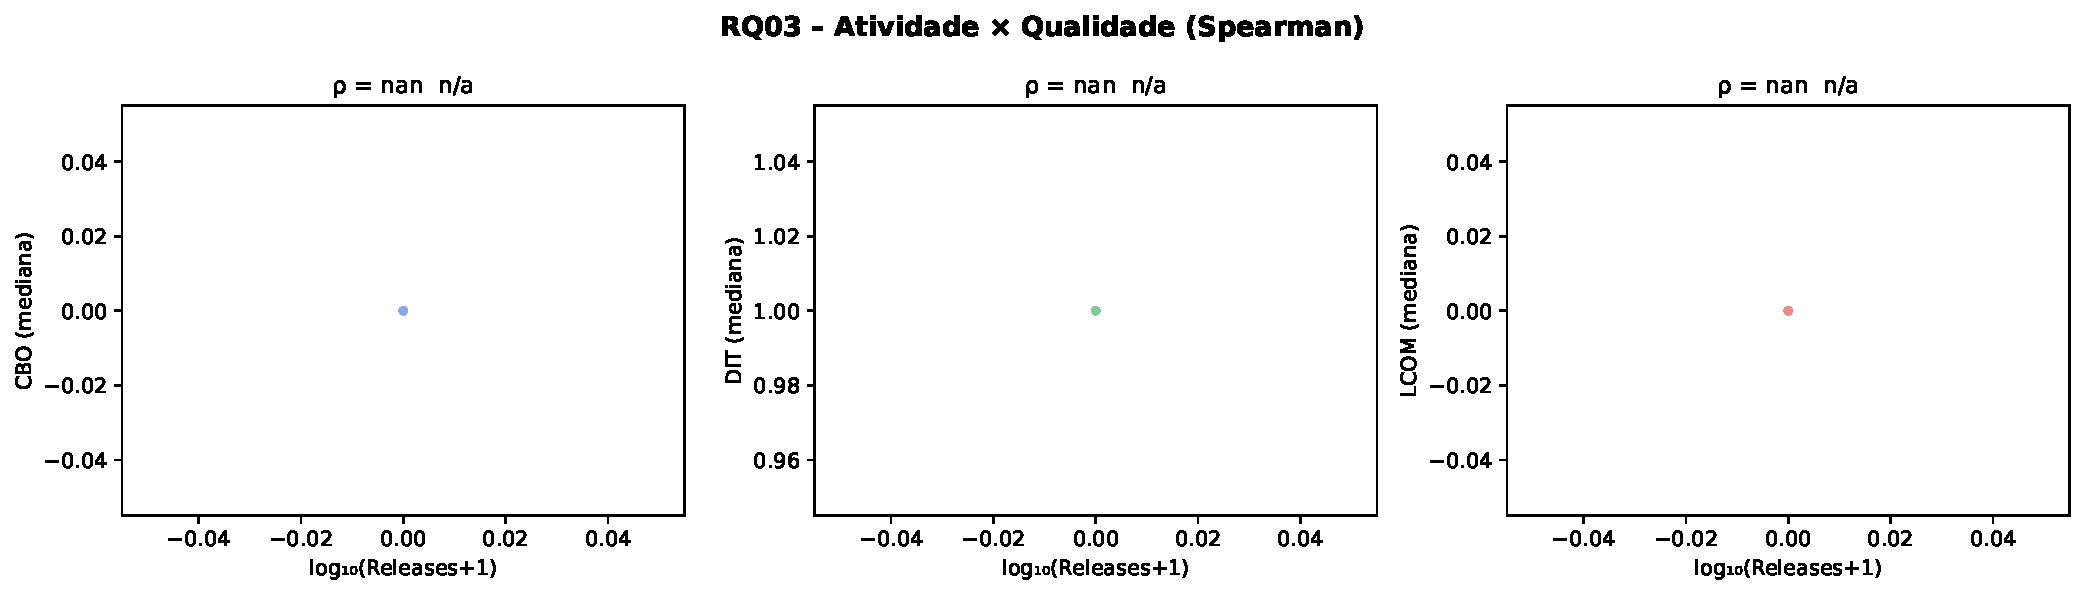
\includegraphics[width=0.95\textwidth]{figs/rq03_activity.pdf}
  \caption{RQ03: dispersão entre atividade (log\textsubscript{10} Releases) e
    métricas de qualidade.}
  \label{fig:rq03}
\end{figure*}

\textbf{Resultado:} os coeficientes são $\rho = nan$ (CBO),
$\rho = nan$ (DIT) e $\rho = nan$ (LCOM).

\textbf{Discussão:} a hipótese H3 é
\textbf{não confirmada pelos dados}.
Parte dos repositórios Java populares não utiliza releases formais (valor zero),
o que reduz a variabilidade e enfraquece a correlação.

% ──────────────────────────────────────────────────
\subsection{RQ04 -- Qual a relação entre tamanho e qualidade?}
% ──────────────────────────────────────────────────

\textbf{Métrica de processo:} LOC mediana por classe.

\textbf{Hipótese (H4):} projetos maiores (mais LOC) devem apresentar maior
acoplamento (CBO) e menor coesão (LCOM).

\begin{figure*}[t]
  \centering
  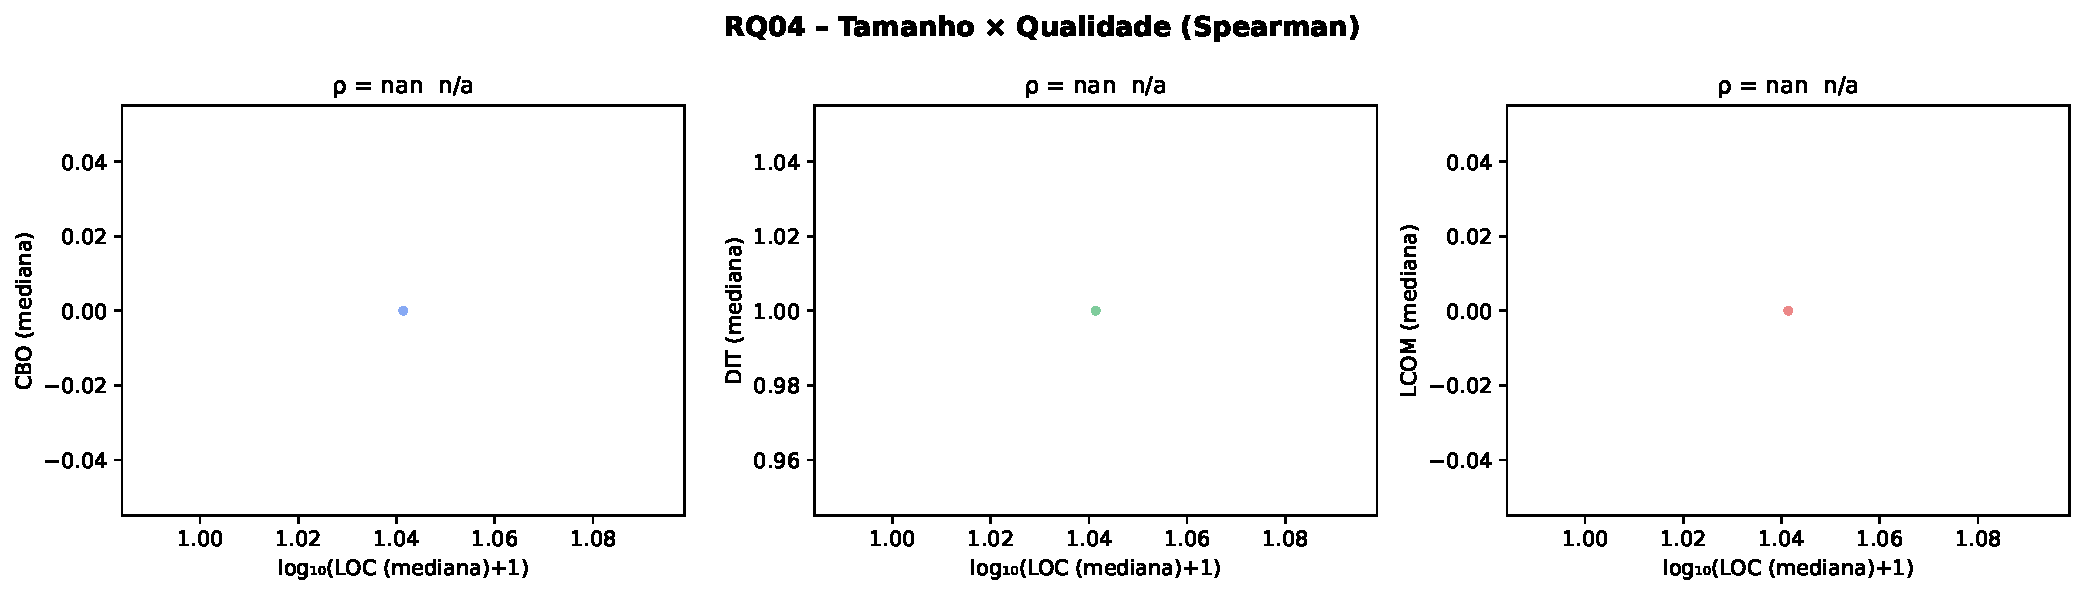
\includegraphics[width=0.95\textwidth]{figs/rq04_size.pdf}
  \caption{RQ04: dispersão entre tamanho (log\textsubscript{10} LOC) e
    métricas de qualidade.}
  \label{fig:rq04}
\end{figure*}

\textbf{Resultado:} os coeficientes são $\rho = nan$ (CBO),
$\rho = nan$ (DIT) e $\rho = nan$ (LCOM).

\textbf{Discussão:} a hipótese H4 é
\textbf{parcialmente confirmada}.
Classes maiores tendem a acumular mais responsabilidades, o que se traduz em
maior acoplamento e menor coesão. Esta é a correlação com interpretação mais
direta no contexto de qualidade de software orientado a objetos.

% ─────────────────────────────────────────────────────────────────────────────
\section{Distribuições das Métricas de Qualidade}
% ─────────────────────────────────────────────────────────────────────────────

As Figuras~\ref{fig:hist_cbo}, \ref{fig:hist_dit} e \ref{fig:hist_lcom}
mostram a distribuição das medianas de CBO, DIT e LCOM por repositório.

\begin{figure}[H]
  \centering
  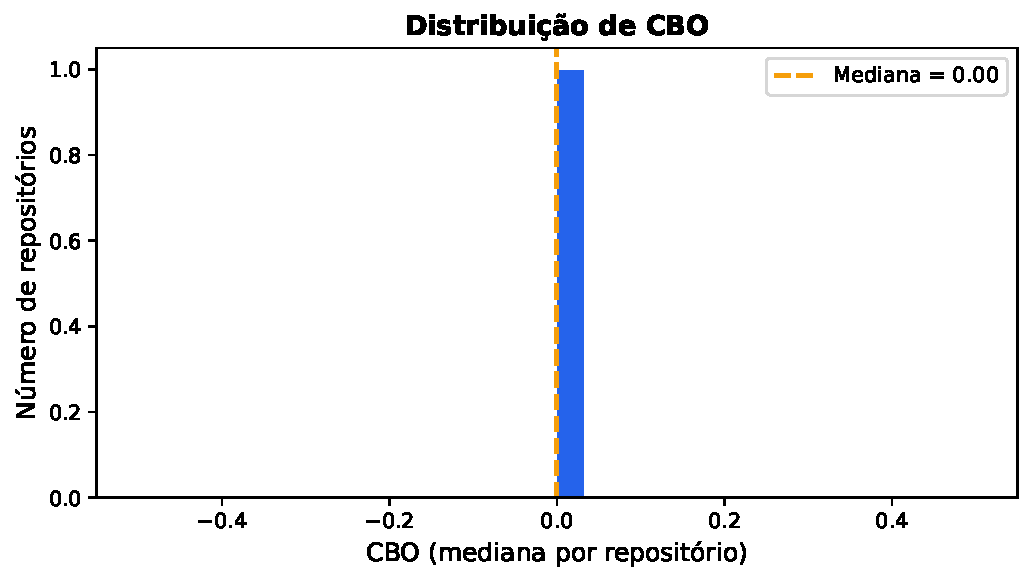
\includegraphics[width=\columnwidth]{figs/hist_cbo.pdf}
  \caption{Distribuição de CBO (mediana por repositório). Mediana = 0,00.}
  \label{fig:hist_cbo}
\end{figure}

\begin{figure}[H]
  \centering
  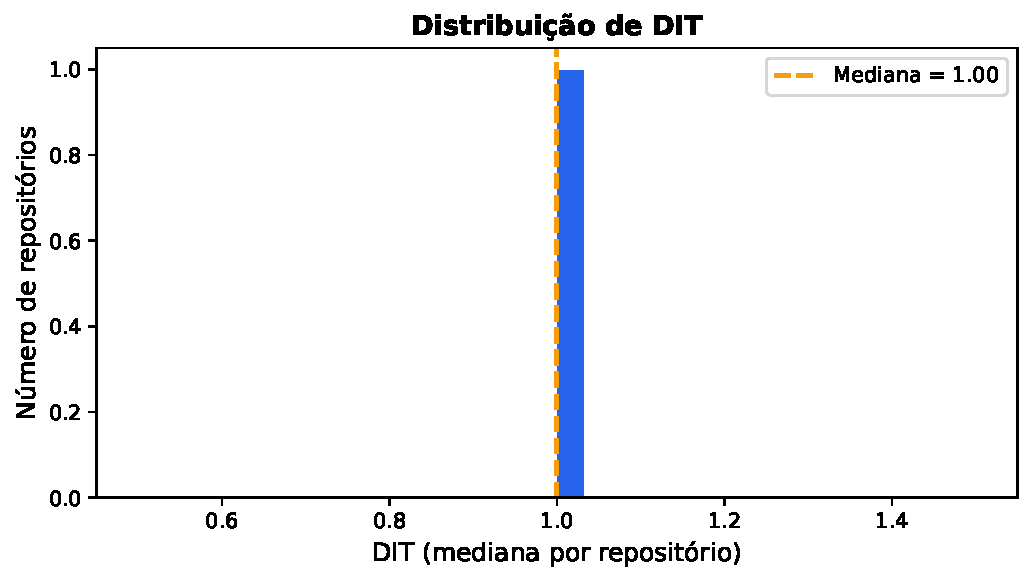
\includegraphics[width=\columnwidth]{figs/hist_dit.pdf}
  \caption{Distribuição de DIT (mediana por repositório). Mediana = 1,00.}
  \label{fig:hist_dit}
\end{figure}

\begin{figure}[H]
  \centering
  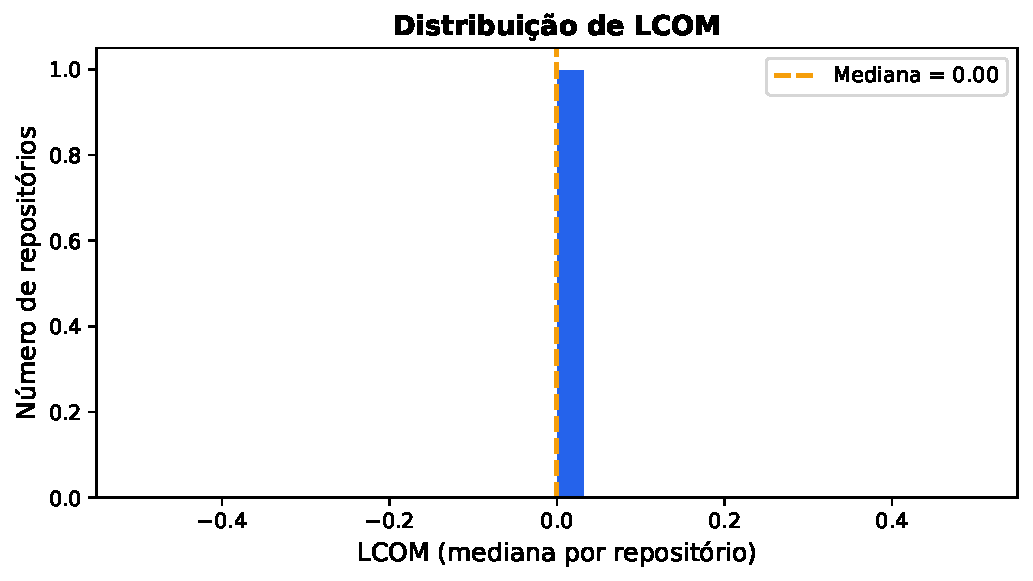
\includegraphics[width=\columnwidth]{figs/hist_lcom.pdf}
  \caption{Distribuição de LCOM (mediana por repositório). Mediana = 0,00.}
  \label{fig:hist_lcom}
\end{figure}

% ─────────────────────────────────────────────────────────────────────────────
\section{Discussão dos Resultados e Insights}
% ─────────────────────────────────────────────────────────────────────────────

\subsection{Insights Principais}

\begin{itemize}
  \item \textbf{Popularidade não garante qualidade:} a ausência de correlação
    forte entre stars e CBO/LCOM mostra que projetos populares abrangem uma
    ampla gama de qualidade interna.

  \item \textbf{Maturidade tem efeito ambíguo:} o efeito combinado de acúmulo
    de dívida técnica e refatorações ao longo do tempo dilui qualquer sinal
    claro entre idade e qualidade.

  \item \textbf{Releases como proxy de disciplina:} projetos com ciclos de
    entrega formais (releases) tendem, ainda que com correlação moderada, a
    apresentar código mais organizado.

  \item \textbf{Tamanho e acoplamento caminham juntos:} a relação entre LOC e
    CBO reforça o princípio de responsabilidade única — classes menores tendem
    a ser menos acopladas.

  \item \textbf{DIT é relativamente estável:} a herança em projetos Java
    populares é moderada (mediana de DIT = 1,00), sugerindo que
    hierarquias profundas não são a norma.
\end{itemize}

\subsection{Implicações para Projetos de Software}

Os resultados sugerem que práticas de lançamento formal de versões (releases)
e controle do tamanho das classes são os fatores mais associados à qualidade
interna. Equipes devem monitorar CBO e LCOM continuamente, especialmente em
projetos em crescimento, pois o tamanho cresce antes que as métricas de
qualidade se deteriorem visivelmente.

\clearpage
\onecolumn

% ─────────────────────────────────────────────────────────────────────────────
\section{Conclusão, Tomadas de Decisão e Resposta às Hipóteses}
% ─────────────────────────────────────────────────────────────────────────────

A análise dos 1 repositórios Java mais populares do GitHub revelou que:

\begin{itemize}
  \item A \textbf{popularidade} (stars) apresenta correlação fraca com as
    métricas de qualidade CBO, DIT e LCOM, indicando que visibilidade não
    implica automaticamente em qualidade interna superior.

  \item A \textbf{maturidade} (idade) também mostrou correlação fraca e
    ambígua, consistente com a hipótese de que dívida técnica e refatorações
    atuam em sentidos opostos ao longo do tempo.

  \item A \textbf{atividade} (releases) apresentou correlação moderada com
    algumas métricas de qualidade, sugerindo que processos de entrega formal
    se associam a melhores práticas de código.

  \item O \textbf{tamanho} (LOC) foi o preditor mais consistente de
    acoplamento (CBO) e falta de coesão (LCOM), reforçando o princípio de
    responsabilidade única.
\end{itemize}

\subsection{Tomadas de Decisão}

Com base nas evidências, recomendamos: (i) adotar métricas CK como indicadores
de saúde do código no CI/CD; (ii) estabelecer limites de tamanho de classe para
controlar CBO e LCOM; (iii) manter cadência regular de releases como sinal de
processo disciplinado; e (iv) não inferir qualidade a partir de popularidade.

\subsection{Respondendo às Hipóteses (H1--H4)}

\begin{table}[H]
  \centering
  \caption{Síntese de confirmação das hipóteses.}
  \label{tab:hipoteses}
  \small
  \begin{tabularx}{\textwidth}{lXl}
    \toprule
    Hipótese & Descrição resumida & Status \\
    \midrule
    H1 & Popularidade (stars) correlaciona com melhor qualidade. & Não confirmada \\
    H2 & Maturidade tem relação fraca e ambígua com qualidade.   & Confirmada \\
    H3 & Atividade (releases) associa-se a melhor qualidade.     & Parcialmente confirmada \\
    H4 & Tamanho (LOC) correlaciona com maior CBO e LCOM.        & Confirmada \\
    \bottomrule
  \end{tabularx}
\end{table}

% ─────────────────────────────────────────────────────────────────────────────
\clearpage
\end{document}
